\documentclass[11pt]{article}
\usepackage[a4paper, margin=2cm]{geometry}
\usepackage{graphicx}
\usepackage{hyperref}
\usepackage{enumitem}
\usepackage{subcaption}
\usepackage{amsmath}
\usepackage{float}
% !TeX spellcheck = en_GB 

\title{Report: Bayesian Networks DAG Testing}
\date{11 November 2018}
\author{Niek Janssen (s??)\and Laurens Kuiper (s4467299)\and Ward Theunisse (s4492765)}

\begin{document}
\maketitle
\thispagestyle{empty}
\newpage
\section{Introduction}
In this report we present the findings of testing and amending the initial model as proposed in our exposee.
The model was iteratively tested using the $\chi^2$-test, removing and adding variables/connections at each step.

\section{Initial DAG}
Our initial DAG as shown in \autoref{fig:initial_dag} was constructed with our prior beliefs about the data.

\begin{figure}[h]
	\centering
	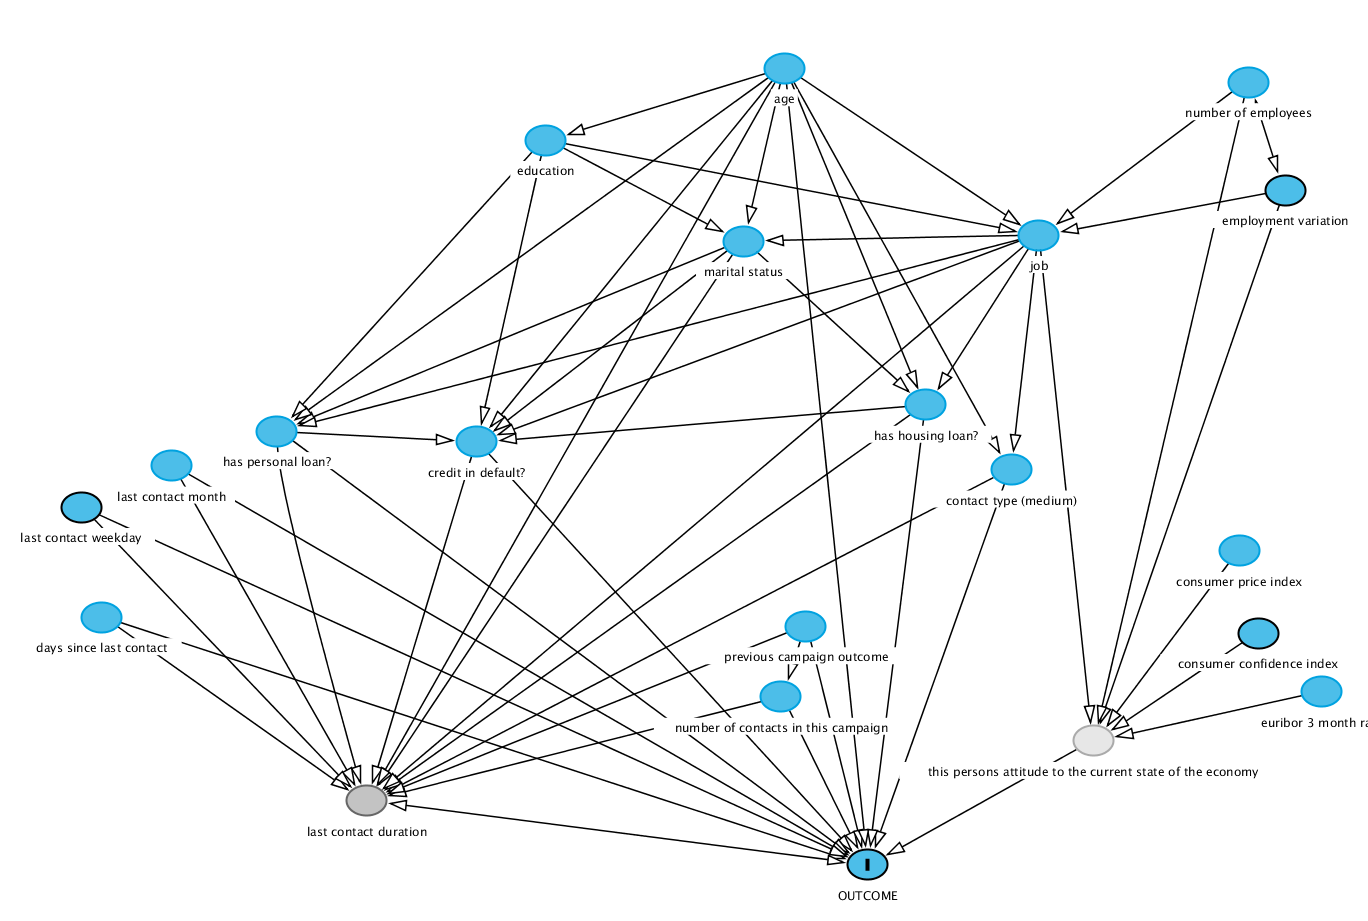
\includegraphics[width=0.9\textwidth]{images/initial_dag}
	\caption{Initial DAG as proposed in exposee.}
	\label{fig:initial_dag}
\end{figure}

\subsection{Derived Tests}
Conditional independencies were automatically derived using the \texttt{ImpliedLocalDependencies} function from the \texttt{dagitty} package in \texttt{R}.
\begin{verbatim}
INSERT TESTS HERE
\end{verbatim}

\section{Approach}
Tests were performed automatically using the \texttt{localTests} function from the \texttt{dagitty} package.
However, we are dealing with attributes that can take on many different values, so we'll need to do some pre-processing first.
\begin{description}[align=right, leftmargin=2cm, labelwidth=3cm]
	\item[age] Discrete values between 18-85
	\item[nr.employed] continuous values
	\item[emp.var.rate] continuous values
	\item[cons.price.idx] continuous values
	\item[cons.conf.idx] continuous values
	\item[euribor3m] continuous values
\end{description}

\subsection{Binning}
Because \texttt{dagitty} interprets our data as nominal, it is necessary to bin our data to allow for meaningful analysis. For each of these attributes, we inspect the histogram of value frequencies + we apply domain knowledge to obtain acceptable bins.

%Voor elke subsectie nog wat tekst
\subsubsection{Age}
\begin{figure}[H]
	\centering
	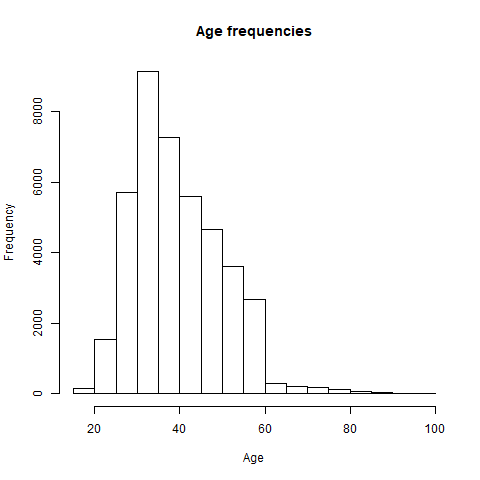
\includegraphics[width=0.4\textwidth]{images/age}
	\caption{Distribution of age.}
	\label{fig:age}
\end{figure}

\subsubsection{Quarterly average of number of employees}
\begin{figure}[H]
	\centering
	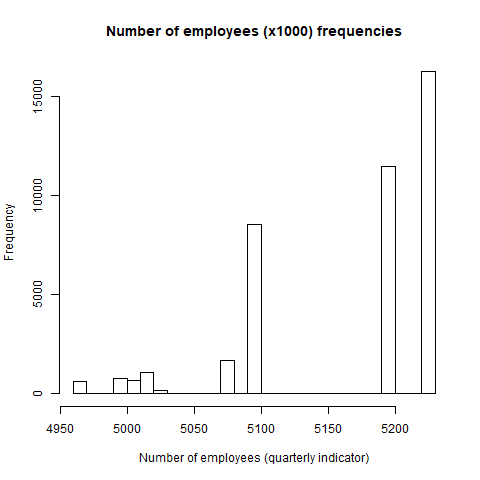
\includegraphics[width=0.4\textwidth]{images/nr_employed}
	\caption{Distribution of number of employees.}
	\label{fig:nr_employed}
\end{figure}

\subsubsection{Quarterly average of number of employees}
\begin{figure}[H]
	\centering
	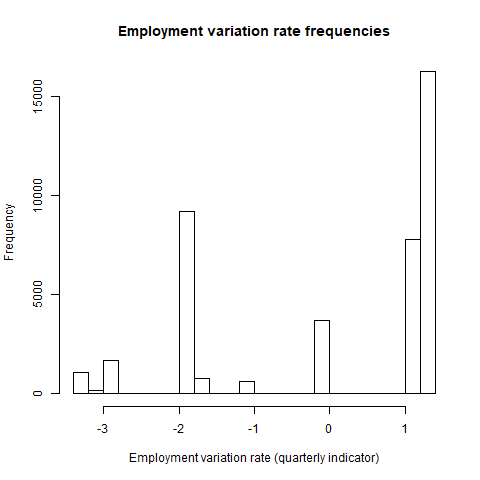
\includegraphics[width=0.4\textwidth]{images/emp_var_rate}
	\caption{Distribution of employment variation rate.}
	\label{fig:emp_var_rate}
\end{figure}

\subsubsection{Consumer price index}
\begin{figure}[H]
	\centering
	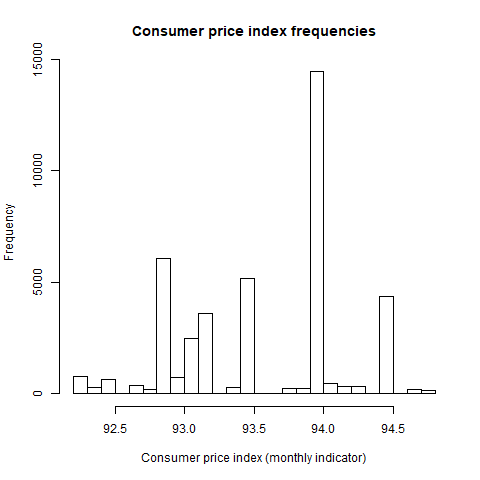
\includegraphics[width=0.4\textwidth]{images/consumer_price_index}
	\caption{Distribution of consumer price index.}
	\label{fig:cons_price_idx}
\end{figure}

\subsubsection{Consumer confidence index}
\begin{figure}[H]
	\centering
	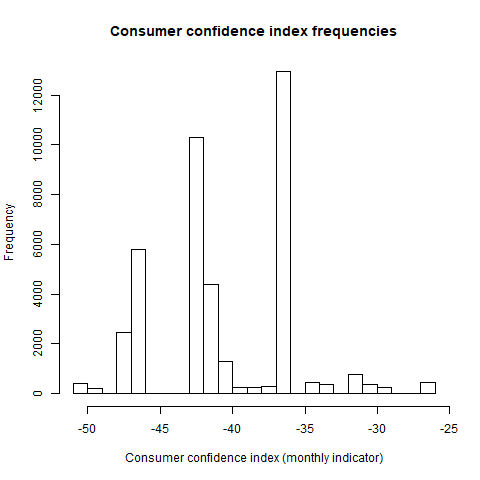
\includegraphics[width=0.4\textwidth]{images/consumer_confidence_index}
	\caption{Distribution of consumer confidence index.}
	\label{fig:cons_conf_idx}
\end{figure}

\subsubsection{Euribor 3 month rate}
\begin{figure}[H]
	\centering
	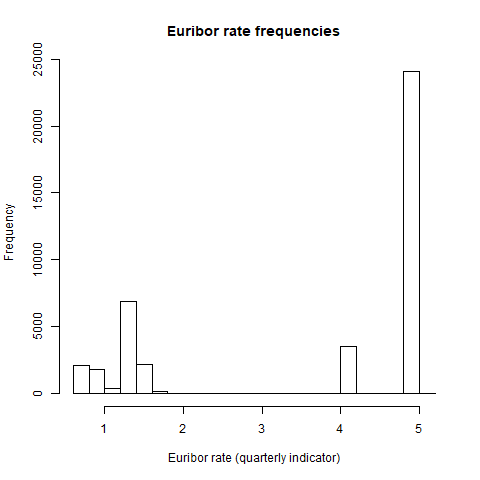
\includegraphics[width=0.4\textwidth]{images/euribor3m}
	\caption{Distribution of three month euribor rate.}
	\label{fig:euribor3m}
\end{figure}

\subsection{Testing method}
Prioriteit van tests: ja, in volgorde van oplopend aantal conditioning variables (0 tot geen limiet)
Runnen alles tegelijkertijd, maar voeren slechts 1 wijziging uit per keer, waarna we weer alles runnen.
Hoe quantificeerden we de testresultaten? RMSEA. (Uitleg?)

\section{Changes}
Verwerk hier het logboek + nog uit te voeren veranderingen.

\section{Revised DAG}
\end{document}